\documentclass{article}
\usepackage[utf8]{inputenc}
\usepackage[T2A]{fontenc}    
\usepackage[english,russian]{babel} 
\usepackage{multicol}
\usepackage[table,xcdraw]{xcolor}
\usepackage{graphicx}
\usepackage{diagbox}
\usepackage{amsmath}
\usepackage{amssymb}
\usepackage{float}
\usepackage{fourier} 
\usepackage{array}
\usepackage{tabularx}
\usepackage{tikz}
\usepackage{lipsum}
\usetikzlibrary{calc,shadings,patterns}
\makeatletter
\tikzset{%
  remember picture with id/.style={%
    remember picture,
    overlay,
    save picture id=#1,
  },
  save picture id/.code={%
    \edef\pgf@temp{#1}%
    \immediate\write\pgfutil@auxout{%
      \noexpand\savepointas{\pgf@temp}{\pgfpictureid}}%
  },
  if picture id/.code args={#1#2#3}{%
    \@ifundefined{save@pt@#1}{%
      \pgfkeysalso{#3}%
    }{
      \pgfkeysalso{#2}%
    }
  }
}

\def\savepointas#1#2{%
  \expandafter\gdef\csname save@pt@#1\endcsname{#2}%
}

\def\tmk@labeldef#1,#2\@nil{%
  \def\tmk@label{#1}%
  \def\tmk@def{#2}%
}

\tikzdeclarecoordinatesystem{pic}{%
  \pgfutil@in@,{#1}%
  \ifpgfutil@in@%
    \tmk@labeldef#1\@nil
  \else
    \tmk@labeldef#1,(0pt,0pt)\@nil
  \fi
  \@ifundefined{save@pt@\tmk@label}{%
    \tikz@scan@one@point\pgfutil@firstofone\tmk@def
  }{%
  \pgfsys@getposition{\csname save@pt@\tmk@label\endcsname}\save@orig@pic%
  \pgfsys@getposition{\pgfpictureid}\save@this@pic%
  \pgf@process{\pgfpointorigin\save@this@pic}%
  \pgf@xa=\pgf@x
  \pgf@ya=\pgf@y
  \pgf@process{\pgfpointorigin\save@orig@pic}%
  \advance\pgf@x by -\pgf@xa
  \advance\pgf@y by -\pgf@ya
  }%
}
\newcommand\tikzmark[2][]{%
\tikz[remember picture with id=#2] {#1;}}
\makeatother



\newcommand\HatchedCell[4][0pt]{%
  \begin{tikzpicture}[overlay,remember picture]%
    \fill[#4] ( $ (pic cs:#2) + (0,1.9ex) $ ) rectangle ( $ (pic cs:#3) + (0pt,-#1*\baselineskip-.8ex) $ );
  \end{tikzpicture}%
}%
\title{Лабораторная работа №7 по информатике}
\author{Ovsyannikov Roman Dmitrievich P3112}
\date{November 2021}

\begin{document}
\begin{center}
\hfill \break
\footnotesize{ФЕДЕРАЛЬНОЕ ГОСУДАРСТВЕННОЕ БЮДЖЕТНОЕ ОБРАЗОВАТЕЛЬНОЕ УЧРЕЖДЕНИЕ}\\ 
\footnotesize{ВЫСШЕГО ПРОФЕССИОНАЛЬНОГО ОБРАЗОВАНИЯ}\\
\footnotesize{{НИУ ИТМО}}\\
\hfill \break
\normalsize{Факультет программной инженерии и компьютерной техники }\\
\hfill \break
\hfill\break
\hfill \break
\hfill \break
\hfill \break
\hfill \break
\hfill \break
\large{Лабораторная работа №7. \\
<<Работа с системой компьютерной вёрстки TEX>>}\\
\hfill \break
\normalsize{Вариант 36}\\
\hfill \break
\hfill \break
\hfill \break
\hfill \break
\hfill \break
\hfill \break
\end{center}
 
\hfill \break
 

\begin{flushright}
\normalsize{ Обучающийся: Овсянников Роман Дмитриевич \\\\
Руководитель: Рудникова Тамара Владимировна}\\\\\\
\end{flushright}

\hfill \break
\hfill \break
\hfill \break
\hfill \break
\hfill \break
\hfill \break
\hfill \break
\hfill \break
\hfill \break
\hfill \break
\begin{center} г. Санкт-Петербург,\\ 2021 г. \end{center}
\thispagestyle{empty}
\newpage

\HatchedCell{start3}{end3}{%
  pattern color=black!70,pattern=north east lines}
  \HatchedCell{start4}{end4}{%
  pattern color=black!70,pattern=north east lines}
  \HatchedCell{start5}{end5}{%
  pattern color=black!70,pattern=north east lines}
  \HatchedCell{start6}{end6}{%
  pattern color=black!70,pattern=north east lines}
  \HatchedCell{start7}{end7}{%
  pattern color=black!70,pattern=north east lines}
  \HatchedCell{start8}{end8}{%
  pattern color=black!70,pattern=north east lines}
  \HatchedCell{start9}{end9}{%
  pattern color=black!70,pattern=north east lines}
  \HatchedCell{start10}{end10}{%
  pattern color=black!70,pattern=north east lines}
\begin{table}[]
\begin{tabular}{|l|l|l|l|l|l|l|l|l|}
\hline
\backslashbox{B}{A}&
  000 &
  001 &
  010 &
  011 &
  100 &
  101 &
  110 &
  111 \\ \hline
000 &
  \multicolumn{1}{!{\hspace*{-0.4pt}\vrule\tikzmark{start3}}c!{\vrule\tikzmark{end3}}}{} &
  1 &
  2/3 &
  2/3 &
  1/7 &
  5/7 &
  3/7 &
  1 \\ \hline
001 &
  1 &
  \multicolumn{1}{!{\hspace*{-0.4pt}\vrule\tikzmark{start4}}c!{\vrule\tikzmark{end4}}}{} &
  2 &
  2 &
  1/3 &
  5/3 &
  1 &
  7/3 \\ \hline
010 &
  3/2 &
  1/2 &
  \multicolumn{1}{!{\hspace*{-0.4pt}\vrule\tikzmark{start5}}c!{\vrule\tikzmark{end5}}}{} &
  1 &
  1 &
  1 &
  3/5 &
  7/5 \\ \hline
011 &
  3/2 &
  1/2 &
  1 &
   \multicolumn{1}{!{\hspace*{-0.4pt}\vrule\tikzmark{start6}}c!{\vrule\tikzmark{end6}}}{} &
  1 &
  1 &
  3 &
  7 \\ \hline
100 &
  7 &
  3 &
  1 &
  1 &
   \multicolumn{1}{!{\hspace*{-0.4pt}\vrule\tikzmark{start7}}c!{\vrule\tikzmark{end7}}}{} &
  1 &
  1/2 &
  3/2 \\ \hline
101 &
  7/5 &
  3/5 &
  1 &
  1 &
  1 &
   \multicolumn{1}{!{\hspace*{-0.4pt}\vrule\tikzmark{start8}}c!{\vrule\tikzmark{end8}}}{} &
  1/2 &
  3/2 \\ \hline
110 &
  7/3 &
  1 &
  5/3 &
  1/3 &
  2 &
  2 &
  \multicolumn{1}{!{\hspace*{-0.4pt}\vrule\tikzmark{start9}}c!{\vrule\tikzmark{end9}}}{} &
  1 \\ \hline
111 &
  1 &
  3/7 &
  5/7 &
  1/7 &
  2/3 &
  2/3 &
  1 &
  \multicolumn{1}{!{\hspace*{-0.4pt}\vrule\tikzmark{start10}}c!{\vrule\tikzmark{end10}}}{}
  \\ \hline
\end{tabular}
\\
\captionof{Таблица 3.}
\end{table}
\begin{multicols}{2}
[\paragraph{Формула Конвея\\}]
Формула Конвея позволяет найти \textit{d(B, A)} при произвольных \textit{B} и \textit{A}, не вычисляя никаких вероятностей. Для того, чтобы объяснить эту формулу, нам нужно определить многочлен Конвея \textit{ $K_{XY}$ } слов \textit{X, Y.}

На рисунке 2 слово \textit{Y} шесть раз записано под словом \textit{X}, причем каждое новое слово \textit{Y} сдвигается на одну позицию вправо по сравнению с предыдущим (для \textit{n-}буквенных слов слово \textit{Y} будет записано под \textit{X} \textit{n} раз). Каждому сдвигу слова \textit{Y} поставим в соответствие число 1 или 0 в зависимости от того, совпадают ли все буквы, находящиеся друг под другом в общих позициях \textit{X} и \textit{Y}, или нет. Полученное таким образом слово (длины \textit{n}) из нулей и единиц называется \textit{корреляцией X} и \textit{Y} и обозначается ⟨X, Y⟩. Так, например, для 2-го сдвига \textit{Y} общие позиции совпадают, поэтому во второй строке на рисунке 2 записана единица --- вторая буква слова ⟨X, Y⟩. В нашем примере

⟨XY⟩ = 010011.\\
В общем случае, пусть ⟨XY⟩ = \textit{$e_{1}$...$e_{n}$} (где \textit{$e_{i}$} --- нули или единицы). Тогда \textit{многочлен Конвея Слов X, Y} определяется так:

\textit{$K_{XY}$(t)=$e_{1}$ + $e_{2}$ + ... + $e_{n}$$t^{n-1}$}\\
В нашем случае \textit{$K_{XY}$(t)=t + $t^{4}$ + $t^{5}$.}

Очень странное определение! Во всяком случае совершенно непонятно, как до него можно было додуматься. Но оно работает --- на нем основана формула Конвея: 

\textit{$$d(B, A)=\frac{K_{AA}(1/2)-K_{AB}(1/2)}{K_{BB}(1/2)-K_{BA}(1/2)}. (*)$$}\\
Можно понять Гарднера, когда он приписывает вывод этой необычной формулы <<потусторонним>> силам: ну магия, и только!

Не останавливаясь пока на выводе формулы (*), поясним, как ею пользоваться. Сначала нужно найти корреляции ⟨AA⟩, ⟨AB⟩, ⟨BB⟩, ⟨BA⟩. Затем по ним написать четьыре многочлена Конвея, в каждом из них подставить \textit{t=1/2} и, наконец, выполнить действия, указанные в правой части формулы (*).

\center{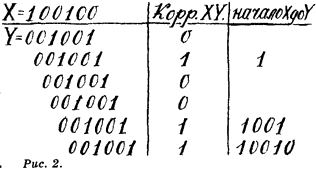
\includegraphics[scale=0.75]{pic}}
\end{multicols}
\newpage
\begin{center}
$A=\large\displaystyle\iint\limits{R}dxdy=\int\limits{-2a}^a\left[\int\limits{y-a}^{a-\frac{y^2}{a}}dx\right]dy=\int\limits{-2a}^a\left[x|{y-a}^{a-\frac{y^2}{a}}\right]dy=\int\limits{-2a}^a\left[a-\frac{y^2}{a}-(y-a)\right]dy=\int\limits{-2a}^a\left(2a-\frac{y^2}{a}-y\right)dy=\left[2ay-\frac{y^3}{3z}-\frac{y^2}{2}\right]\bigg|{-2a}^a=\left(2a^2-\frac{a^3}{3a}-\frac{a^2}{2}\right)-\left(-4a^2+\frac{8a^3}{3a}-\frac{4a^2}{2}\right)=\frac{9a^2}{2}$
\end{center}


\end{document}
